\chapter{Desarrollo}
\label{chap:cap3}
\section{Experimentos}
\subsection{Tama�o del bloque de memoria}
\begin{verbatim}
$ ./archivos_marcados_b3.sh
$ ./tam_bloque_b2.sh
$ dd if=datos/datosfin.txt of=/media/cesar/4F35-D764/datosfin
$ cp datos2/datos1.txt /media/cesar/4F35-D764/datos1.txt
$ cp datos2/datos1.txt /media/cesar/4F35-D764/datos2.txt
$ sudo dd if=/dev/sdb1 of=tambloque.iso
\end{verbatim}


\subsection{Tabla de nombres}



\subsection{Movimiendo de datos entre sectores}

\subsection{Vida �til}

Despu�s de varias pruebas con el script \verb|flash_b2.sh| y \verb|flash_b3.sh| no conseguimos el resultado esperado, que es obtener datos para generar una gr�fica que muestre como disminuye la capacidad seg�n se van deteriorando bloques de memoria.

Al principio pensamos que como este tipo de memorias tienen bloques reservados para que el deterioro de la capacidad no se vea reflejado, pues nosotros tampoco er�mos capaces de verlo. Entonces hicimos pruebas m�s largas para evitar este posible problema. Pero solo conseguimos que la memoria diese errores de entrada/salida y la memoria dejase de estar accesible \ref{fig:errorlectura}.

En una prueba con una memoria con este estado inicial:
\begin{verbatim}
$ df --block-size=KB
Filesystem      1kB-blocks        Used   Available Use% Mounted on
/dev/sde1        3924005kB         5kB   3924000kB   1% /media/cesar/usb3
\end{verbatim}

\begin{figure}[h!]
	\centering
		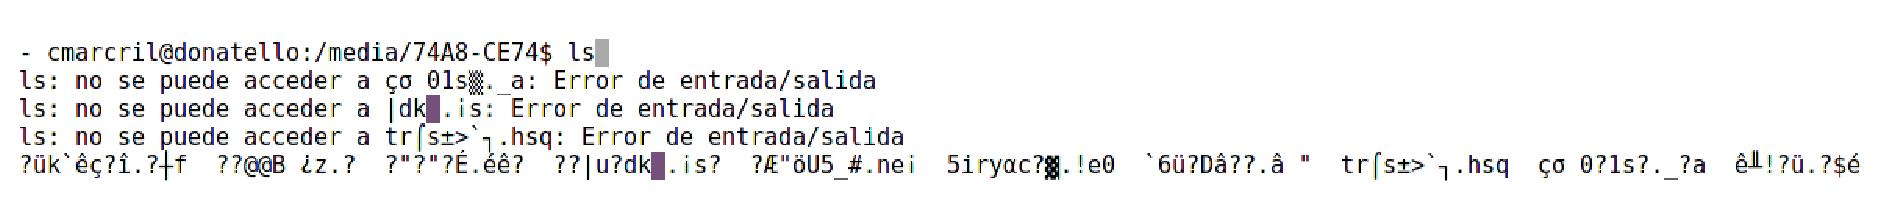
\includegraphics[height=25mm,width=1\textwidth,natwidth=610,natheight=642]{fig/errorlectura.eps}
	\caption{\emph{Errores de lectura en la memoria}}
        \label{fig:errorlectura}
\end{figure}

Estas fueron las �ltimas l�neas del log donde vamos apuntado cada ciclo de escritura/borrado:
\begin{verbatim}
$ tail stam.txt
Filesystem     1K-blocks      Used Available Use% Mounted on
/dev/sde1      3924005kB 2189669kB 1734337kB  56% /media/74A8-CE74
vuelta  50356019
/dev/sde1      3924005kB 2189669kB 1734337kB  56% /media/74A8-CE74
vuelta  50356020
/dev/sde1      3924005kB 2189669kB 1734337kB  56% /media/74A8-CE74
vuelta  50356021
\end{verbatim}
Lo que quiere decir que 

Tambi�n buscamos errores en el syslog del kernel y esta fue su salida:
\begin{verbatim}
kern.log:May 15 19:32:56 donatello kernel: [1699652.958924] FAT: Filesystem error (dev sde1)
kern.log:May 15 19:32:56 donatello kernel: [1699652.972408] FAT: Filesystem error (dev sde1)
kern.log:May 15 19:32:56 donatello kernel: [1699652.972426] FAT: Filesystem error (dev sde1)
kern.log:May 15 19:51:50 donatello kernel: [1700786.560947] sd 12:0:0:0: [sde] Attached SCSI removable disk
messages:May 15 19:51:50 donatello kernel: [1700786.560947] sd 12:0:0:0: [sde] Attached SCSI removable disk
syslog:May 15 19:32:56 donatello kernel: [1699652.958924] FAT: Filesystem error (dev sde1)
syslog:May 15 19:32:56 donatello kernel: [1699652.972408] FAT: Filesystem error (dev sde1)
syslog:May 15 19:32:56 donatello kernel: [1699652.972426] FAT: Filesystem error (dev sde1)
syslog:May 15 19:51:50 donatello kernel: [1700786.560947] sd 12:0:0:0: [sde] Attached SCSI removable disk
\end{verbatim}
Lo que nos da a suponer que algo del sistema de ficheros o del controlador se ha corrompido, pero la memoria sigue intacta.

En otros dos casos, no conseguimos obtener datos en el momento que la memoria empez� a fallar pero quedo 
\begin{verbatim}
[ 4673.313154] usb 3-1: new high-speed USB device number 3 using ehci-pci
[ 4673.444924] usb-storage 3-1:1.0: USB Mass Storage device detected
[ 4673.446328] scsi3 : usb-storage 3-1:1.0
\end{verbatim}

\begin{verbatim}
# fdisk /dev/sdc
Device does not contain a recognized partition table.
Created a new DOS disklabel with disk identifier 0x1670df5f.
\end{verbatim}

\begin{verbatim}
$ df
Filesystem     1K-blocks      Used Available Use% Mounted on
/dev/sdc1        3831940    716640   3115300  19% /media/cesar/usb1
\end{verbatim}


Vamos a llenar el dispositivo con un fichero con \textit{00}. Despu�s borramos el archivo y copiamos un archivo de 64K que contiene \textit{CC}. Hacemos una imagen \verb|.iso| de la memoria, borramos el fichero, creamos otra imagen, volvemos a copiar el mismo archivo y hacemos otra imagen del dispositivo.
\begin{verbatim}
$ ./archivos_marcados_b3.sh
$ ./tam_bloque_b2.sh
$ dd if=datos/datosfin.txt of=/media/cesar/4F35-D764/datosfin.txt
$ rm /media/cesar/4F35-D764/datosfin.txt
$ cp datos2/datos16.txt /media/cesar/4F35-D764/
$ sudo dd if=/dev/sdb1 of=datos16.iso
$ rm /media/cesar/4F35-D764/datos16.txt
$ sudo dd if=/dev/sdb1 of=datos16borrado.iso
$ cp datos2/datos16.txt /media/cesar/4F35-D764/
$ sudo dd if=/dev/sdb1 of=datos16copiado.iso
\end{verbatim}

Con \verb|bless| hemos visto que los datos siguen estado despu�s de haber borrado el fichero. Pero \verb|md5sum| nos dice que las im�genes sin distintas, as� que vamos a crear ficheros de texto con \verb|hexdum| para poder comparar las im�genes con \verb|meld|.
\begin{verbatim}
$ md5sum *
5b47c568523dbb3bb3128e3f4193148d  datos16.iso
5704c3cc3b5264aecfc5e5a4a54f0bf5  datos16borrado.iso
9fbc3200e1f61767c5c0da7353fe1c72  datos16copiado.iso
\end{verbatim}


\section{C�digo}
\verb|archivos_marcados_b3.sh|
\begin{lstlisting}
#
# Crea ficheros de todos los tama�os posibles hasta llegar a 'valor_final'
#
valor_final=3907388
((tamfinal=valor_final*1024))

aux=2
cont=0
while [ $aux -le  $tamfinal ]; do

	((aux=aux+aux))
	((cont++))
done

echo "auxiliar" $aux
echo "contado" $cont
rm datos/*
echo -e -n "\x00" > datos/datos0.txt

((aux=cont))

echo "vamos a contar desde 1 a " $aux

for (( a=1 ; a<=aux ; a++ ))
do
	((b=a-1))
	cat datos/datos$b.txt > datos/datos$a.txt
	cat datos/datos$b.txt >> datos/datos$a.txt
	echo $b
	echo $a
done
\end{lstlisting}


\verb|flash_b2.sh|
\begin{lstlisting}
#
# 
#
dispo="4E06-0AB9"
sdd="sdb"
rm stam.txt	
for (( b=0 ; b<999999999999999999999 ;b++))
do
	let vueltas=$b

for (( a=1 ; a<3 ; a++ ))
do
	echo "numero serie ${b}_${a}"
	echo -e -n "numero serie ${b}_${a}" > datos/${b}_${a}datos.txt
	for (( c=1 ; c<200 ; c++ ))
	do
		echo -e -n "numero serie ${b}_${a}" >> 
datos/${b}_${a}datos.txt
	done
	#cat datos/datos.txt >> datos/${b}_${a}datos.txt
	#echo -e -n "numero serie ${b}_${a}" >> datos/${b}_${a}datos.txt
	dd if=datos/${b}_${a}datos.txt 
of=/media/${dispo}/${b}_${a}datos.txt
	rm datos/*_*datos.txt
done

rm -f /media/${dispo}/*datos.txt

df --block-size=KB | grep ${sdd} >> stam.txt
#cut -c32-52 tam.txt >> stam.txt

frase="vuelta "
echo "$frase $vueltas" >> stam.txt
echo " " >> stam.txt

#sudo umount /media/usb0
#sudo mount /dev/sdc1 /media/usb0

done
\end{lstlisting}


\verb|flash_b3.sh|
\begin{lstlisting}
#
# Crea un fichero con un texto reconocible y su numero de serie
#
rm stam.txt
rm diff.txt
for (( b=0 ; b<10 ;b++))
do
	let vueltas=$b

for (( a=1 ; a<3 ; a++ ))
do
	echo "numero serie ${b}_${a}"
	echo -e -n "En un lugar de la Mancha, de cuyo nombre no quiero 
acordarme, no ha mucho tiempo que viv�a un hidalgo de los de lanza en astillero, adarga antigua, roc�n flaco y galgo corredor. Una olla de algo m�s vaca que carnero, salpic�n las m�s 
noches, duelos y quebrantos los s�bados, lentejas los viernes, alg�n palomino de a�adidura los domingos, consum�an las tres partes de su 
hacienda. El resto della conclu�an sayo de velarte, calzas de velludo para las fiestas con sus pantuflos de lo mismo, los d�as de entre 
semana se honraba con su vellori de lo m�s fino. Ten�a en su casa una ama que pasaba de los cuarenta, y una sobrina que no llegaba a los 
veinte, y un mozo de campo y plaza, que as� ensillaba el roc�n como tomaba la podadera. Frisaba la edad de nuestro hidalgo con los 
cincuenta a�os, era de complexi�n recia, seco de carnes, enjuto de rostro; gran madrugador y amigo de la caza. Quieren decir que ten�a el 
sobrenombre de Quijada o Quesada (que en esto hay alguna diferencia en los autores que deste caso escriben), aunque por conjeturas 
veros�miles se deja entender que se llama Quijana; pero esto importa poco a nuestro cuento; basta que en la narraci�n d�l no se salga un 
punto de la verdad. ${b}_${a}" > datos/${b}_${a}datos.txt
	#cat datos/datos.txt >> datos/${b}_${a}datos.txt
	#echo -e -n "numero serie ${b}_${a}" >> datos/${b}_${a}datos.txt
	dd if=datos/${b}_${a}datos.txt of=/media/usb0/${b}_${a}datos.txt
	rm datos/*_*datos.txt
done

dd if=/dev/sdc1 of=copias/${b}.iso

echo "vuelta ${b}" >> diff.txt

if (($b != 0 ))
then
((c=b-1))
cmp -l copias/${b}.iso copias/${c}.iso >> diff.txt
fi

echo "" >> diff.txt

rm -f /media/usb0/*datos.txt

df --block-size=KB | grep sdc1 > tam.txt
cut -c32-52 tam.txt >> stam.txt

frase="vuelta "
echo "$frase $vueltas" >> stam.txt
echo " " >> stam.txt

done
\end{lstlisting}

\verb|mount.sh|
\begin{lstlisting}
rm md5.txt

for (( a=1 ; a<999999999999999 ; a++ ))
do
	sudo umount /media/usb0
	sudo mount /dev/sdb1 /media/usb0
	echo "$a" >> md5.txt
	dd if=/dev/sdb1 | md5sum >> md5.txt

done
\end{lstlisting}

\verb|tam_bloque_b1.sh|
\begin{lstlisting}
df --block-size=KiB | grep sdb1 > tam.txt
tam_final=$(cut -c56-63 tam.txt)
echo $tam_final
((valor_final=tam_final-6))
((valor_final_bits=valor_final*1024))
echo "valor final" $valor_final_bits
final_binario=$(echo "obase=2; $valor_final_bits"| bc)
echo $final_binario > long.txt
echo "valor en binario" $final_binario
long=${#final_binario}


((long--))

total=0

((exp=long))

for ((a=1;a<=long;a++))
do
bit=$(cut -c$a-$a long.txt)
#echo "a="$a "bit sacado de long.txt" $bit
if((bit==1))
then
	((exponente=2**exp))
#	echo "exponente" $exp
	echo $exp $exponente
	((total=total+exponente))
	
	cat datos/datos$exp.txt >> datos/datosfin.txt
fi
((exp--))
done

echo $total
\end{lstlisting}

\verb|tam_bloque_b2.sh|
\begin{lstlisting}
((valor_final=3907388))
#((valor_final=3907388/4))
((valor_final_bits=valor_final*1024))
echo "valor final" $valor_final_bits
final_binario=$(echo "obase=2; $valor_final_bits"| bc)
echo $final_binario > long.txt
echo "valor en binario" $final_binario
long=${#final_binario}


((long--))

total=0

((exp=long))
rm datos/datosfin.txt
for ((a=1;a<=long;a++))
do
bit=$(cut -c$a-$a long.txt)
#echo "a="$a "bit sacado de long.txt" $bit
if((bit==1))
then
	((exponente=2**exp))
#	echo "exponente" $exp
	echo $exp $exponente
	((total=total+exponente))
	
	cat datos/datos$exp.txt >> datos/datosfin.txt
fi
((exp--))
done

echo $total
\end{lstlisting}
